\documentclass[11pt]{article}
\usepackage[letterpaper,margin=0.9in]{geometry}
\usepackage{amsmath,amssymb,amsthm}
\usepackage{pgfplots}
\pgfplotsset{compat=1.18}
\usepackage{tcolorbox}
\usepackage[colorlinks,allcolors=blue!50!black]{hyperref}
% LaTeX's defaults; Debian's TeX Live 2023 leaves these at 0 ("u-nique")
\lefthyphenmin=2 \righthyphenmin=3
% the US patterns allow "hyperg-amous" and "hypog-amous"
\hyphenation{hy-per-ga-mous hy-po-ga-mous hy-per-ga-my hy-po-ga-my}
% stretch a tight paragraph instead of overflowing (two-digit citations)
\emergencystretch=1em

\newtheorem{theorem}{Theorem}[section]
\newtheorem{lemma}[theorem]{Lemma}
\newtheorem{proposition}[theorem]{Proposition}
\newtheorem{corollary}[theorem]{Corollary}
\theoremstyle{definition}
\newtheorem{definition}[theorem]{Definition}
\newtheorem{example}[theorem]{Example}
\theoremstyle{remark}
\newtheorem{remark}[theorem]{Remark}

\newcommand{\M}{\mathfrak{M}}
\newcommand{\W}{\mathfrak{W}}
\newcommand{\X}{\mathcal{X}}
\newcommand{\Y}{\mathcal{Y}}
\newcommand{\C}{\mathcal{C}}
\newcommand{\R}{\mathbb{R}}
\newcommand{\D}{\mathsf{D}}
\newcommand{\Hy}{\mathsf{H}}
\DeclareMathOperator{\Unif}{Unif}
\DeclareMathOperator{\Leb}{Leb}
\DeclareMathOperator{\Ent}{Ent}
\DeclareMathOperator{\Var}{Var}

\title{
  \textbf{Hypergamy Is Solved}\\[0.2em]
  \large Feasibility, Deficit, and Equilibrium in Status-Ordered
  Matching Markets
}
\author{}
\date{October 23, 2026}

\begin{document}
\maketitle

\begin{abstract}
  Hypergamy, the tendency to form unions with a partner of higher
  status, is usually argued about as a behavioral claim. We instead
  model the marriage market as a coupling problem between Borel
  probability measures on Polish type spaces and show that, absent
  taste heterogeneity, every aggregate question about hypergamy
  reduces to a question about two marginal distributions. We prove:
  (i) universal hypergamy is feasible if and only if one status
  distribution first-order stochastically dominates the other
  (Strassen); (ii) otherwise the minimal unmatched mass is the
  \emph{Hypergamy Deficit} $\D = \sup_t(G_\W - G_\M)^+$ (a continuum
  Hall marriage theorem); (iii) no behavioral strategy changes any of
  this (\emph{Cope Invariance}), and status gains are zero-sum in rank
  (\emph{Conservation of Rank}); (iv) under status-ranked preferences
  the unique Gale--Shapley stable matching is positive assortative,
  and under Becker--Shapley--Shubik transferable utility it is the
  comonotone optimal transport plan, with the Choo--Siow entropic
  relaxation tending to random matching as taste shocks grow. Height is
  our worked example: for equal variances the deficit for a required
  height gap has a closed form that vanishes up to the mean difference
  of about 14 cm, and the height preference online daters reveal is
  relative, which the market can satisfy. We chose height because it is
  measurable, not because it matters most, and review what else people
  weight: kindness and intelligence in stated long-term preferences, the
  relationship itself in predicting relationship quality, and looks in
  stated short-term preferences. With several traits, checklist
  requirements shrink the eligible pool multiplicatively when traits are
  independent, trade-offs reduce to a scalar index, and a required rank
  gap $\delta$ leaves exactly $\delta$ of one side unmatched. We model
  partner history as a comparison effect, which applies to both sexes,
  and show that, for an average new partner, one ex remembered a standard
  deviation better than they were costs more than four ordinary ones.
\end{abstract}

\section{The Marriage Market as a Measure Space}

\begin{definition}[Market]
  A \emph{marriage market} is a tuple $(\X,\Y,\mu,\nu,s)$ where $\X$
  and $\Y$ are Polish spaces of agent types for the two sides $\M$
  and $\W$, $\mu\in\mathcal{P}(\X)$ and $\nu\in\mathcal{P}(\Y)$ are
  Borel probability measures describing the populations, and
  $s:\X\sqcup\Y\to\R$ is a measurable \emph{status functional}
  (height, income, education, follower count, or any scalar index
  thereof). We write $\mu_s = s_\#\mu$ and $\nu_s = s_\#\nu$ for the
  pushforward status distributions, with CDFs $F_\M, F_\W$ and
  survival functions $G_\M(t) = \mu(s\ge t)$, $G_\W(t) = \nu(s\ge t)$.
\end{definition}

\begin{definition}[Matching]
  A \emph{matching} is a coupling $\pi\in\Pi(\mu,\nu)$, i.e.\ a Borel
  probability measure on $\X\times\Y$ with marginals $\mu$ and $\nu$.
  A \emph{partial matching} is a sub-coupling: a measure $\pi$ with
  $(p_1)_\#\pi\le\mu$ and $(p_2)_\#\pi\le\nu$. Its \emph{mass} $|\pi|
  = \pi(\X\times\Y)$ is the amount of each side that is matched.
\end{definition}

\begin{definition}[Hypergamy]
  A partial matching $\pi$ is \emph{hypergamous for} $\W$ if
  $\pi(\{s(x)\ge s(y)\}) = |\pi|$, and \emph{strictly hypergamous} if
  the inequality is strict $\pi$-a.e. The \emph{hypergamy index} is
  $\Hy(\pi) = \pi(\{s(x) > s(y)\})$ and the \emph{hypogamy index} is
  $\Hy^{\downarrow}(\pi) = \pi(\{s(x) < s(y)\})$.
\end{definition}

\begin{remark}
  Every definition is symmetric under exchanging $(\X,\mu)$ with
  $(\Y,\nu)$. Conventional usage applies hypergamy to $\W$, and we
  follow that convention for notation only. No result depends on
  which side is labeled which, and the reader is free to swap the
  letters if it makes them feel better.
\end{remark}

\section{Who Can Marry Up? Feasibility and the Deficit}

\begin{theorem}[Hypergamy Feasibility]\label{thm:feas}
  A hypergamous matching $\pi\in\Pi(\mu,\nu)$ exists if and only if
  $\mu_s$ first-order stochastically dominates $\nu_s$:
  \begin{equation}\label{eq:fsd}
    G_\M(t) \ge G_\W(t) \qquad \text{for all } t\in\R.
  \end{equation}
\end{theorem}

\begin{proof}
  ($\Rightarrow$) If $\pi$ is hypergamous then $\{s(y)\ge
  t\}\subseteq\{s(x)\ge t\}$ up to a $\pi$-null set, so $G_\W(t) =
  \pi(s(y)\ge t) \le \pi(s(x)\ge t) = G_\M(t)$. ($\Leftarrow$) With
  generalized inverses $F^{-1}(u) = \inf\{t : F(t)\ge u\}$, condition
  \eqref{eq:fsd} gives $F_\M^{-1}(u)\ge F_\W^{-1}(u)$ for all $u$, so
  for $U\sim\Unif(0,1)$ the pair $(F_\M^{-1}(U), F_\W^{-1}(U))$
  couples $(\mu_s,\nu_s)$ on $\{a\ge b\}$. Lift to $\X\times\Y$ by
  disintegrating $\mu,\nu$ along the fibers of $s$ (possible since
  the spaces are Polish). This is the one-dimensional case of
  Strassen's theorem~\cite{strassen}.
\end{proof}

When \eqref{eq:fsd} fails, someone has to marry down or stay single.
We compute exactly how many. Allow general masses $\mu(\X) = m$,
$\nu(\Y) = w$ and let $\C = \{(x,y) : s(x)\ge s(y)\}$.

\begin{theorem}[Hypergamy Deficit Formula]\label{thm:deficit}
  The maximal mass of a partial matching supported on $\C$ is
  \begin{equation}
    \max_{\pi(\C^c)=0} |\pi| = w - \D, \qquad \D := \sup_{t\in\R}
    \bigl(\nu(s\ge t) - \mu(s\ge t)\bigr)^+.
  \end{equation}
  $\D$ is the minimal mass of $\W$ left unmatched if every union is hypergamous.
\end{theorem}

\begin{proof}
  \emph{Upper bound.} Agents in $\W$ with $s(y)\ge t$ are compatible
  only with $\{x : s(x)\ge t\}$, so at least $\nu(s\ge t) - \mu(s\ge
  t)$ of them are unmatched; take the supremum. \emph{Achievability.}
  Leave the top $\D$ of $\W$ by status unmatched, splitting an atom if
  necessary, and use only the top $w-\D\le m$ of $\M$. These women and
  men have survival functions $(G_\W-\D)^+$ and $\min(G_\M,w-\D)$, and
  the second dominates the first because $G_\W-G_\M\le\D$ and
  $G_\W\le w$, so Theorem~\ref{thm:feas}, rescaled to mass $w-\D$,
  matches them hypergamously. For finitely supported measures this is
  the deficiency form of Hall's theorem: compatibility is
  \emph{nested}, so Hall's condition need only be checked on upper
  sets.
\end{proof}

\begin{corollary}
  $\D = 0$ iff \eqref{eq:fsd} holds (when $m = w$), and
  $\D\ge(w-m)^+$. A skewed sex ratio is a lower bound on the deficit;
  everything above it is caused by the shape of the distributions.
\end{corollary}

\begin{example}\label{ex:beta}
  Let $\mu_s = \Unif[0,1]$ and $\nu_s = \mathrm{Beta}(2,1)$, so
  $G_\M(t) = 1-t$ and $G_\W(t) = 1-t^2$. Then $\D = \sup_t(t-t^2) =
  \frac14$ at $t^* = \frac12$. With a perfectly balanced sex ratio,
  one quarter of $\W$ still cannot be matched hypergamously, and the
  bottleneck sits exactly at the median of $\M$.
\end{example}

\section{Application: The Six-Foot Rule}\label{sec:sixfoot}

Height is the cleanest test case: scalar, observable, approximately
Gaussian within each sex, and the subject of strongly held opinions. It
is chosen for convenience, not because it matters most, and
Section~\ref{sec:matters} reviews what else does.
Take $s ={}$ height in cm with $\mu_s = N(m_\M,\sigma_\M^2)$ and
$\nu_s = N(m_\W,\sigma_\W^2)$. We calibrate to US adult means from
NHANES 2015--2018~\cite{fryar}, $m_\M\approx175.3$ and
$m_\W\approx161.3$, write $\Delta m\approx14.0$, and take
$\sigma_\M = 7.6$ and $\sigma_\W = 7.1$. The report gives percentiles
rather than standard deviations, and its percentiles imply 7.4--7.5
and 6.9--7.1.

\begin{proposition}[The $-37.5$ cm Theorem]\label{prop:crossing}
  For Gaussian marginals with $\sigma_\M\ne\sigma_\W$, the survival
  functions cross exactly once, at
  \begin{equation}
    t_\times = \frac{\sigma_\M m_\W - \sigma_\W m_\M}{\sigma_\M -
    \sigma_\W} \approx -37.5\,\mathrm{cm}.
  \end{equation}
  Hence \eqref{eq:fsd} fails only on $(-\infty,t_\times)$ and $\D(0)
  < 10^{-150}$.
\end{proposition}

\begin{proof}
  $G_\M(t) = G_\W(t)$ iff $(t-m_\M)/\sigma_\M = (t-m_\W)/\sigma_\W$,
  a linear equation with unique root $t_\times$. Above it, $\M$ has
  the smaller standardized score, so $G_\M > G_\W$. Below it the gap
  is at most $\Phi$ of a standardized value near $-28$.
\end{proof}

\begin{remark}
  ``He must be taller than me'' is therefore feasible for every human
  of positive height. The only obstruction occurs below $-37.5$ cm, a
  region the author was unable to sample. Other readings of the
  report's percentiles move the crossing anywhere from $-6$ to $-108$
  cm, which the author did not sample either.
\end{remark}

Now require a gap. A union satisfies the \emph{$\delta$-rule} if
$s(x)\ge s(y)+\delta$. Shifting $\nu_s$ by $\delta$ reduces this to
Theorem~\ref{thm:deficit}, so $\D(\delta) = \sup_t(G_\W(t) - G_\M(t+\delta))^+$.

\begin{theorem}[Closed-Form Height Deficit]
  If $\sigma_\M = \sigma_\W = \sigma$, then
  \begin{equation}
    \D(\delta) = \left(2\,\Phi\!\left(\frac{\delta-\Delta
    m}{2\sigma}\right) - 1\right)^{+}.
  \end{equation}
  $\D$ vanishes iff $\delta\le\Delta m$, and is concave increasing
  beyond it with initial slope $(\sigma\sqrt{2\pi})^{-1}$, or $5.4\%$
  per~\textup{cm} at the pooled $\sigma = 7.35$~\textup{cm}.
\end{theorem}

\begin{proof}
  With $z = (t-m_\W)/\sigma$ and $c = (\delta-\Delta m)/\sigma$, the
  gap is $\Phi(z+c) - \Phi(z)$, the Gaussian mass of an interval of
  length $c$. For $c > 0$ it is maximized by centering the interval
  at the mode, $z = -c/2$, giving $2\Phi(c/2) - 1$. Its
  $\delta$-derivative $\varphi(c/2)/\sigma$ is decreasing in $c$.
\end{proof}

\begin{figure}[ht]
  \centering
  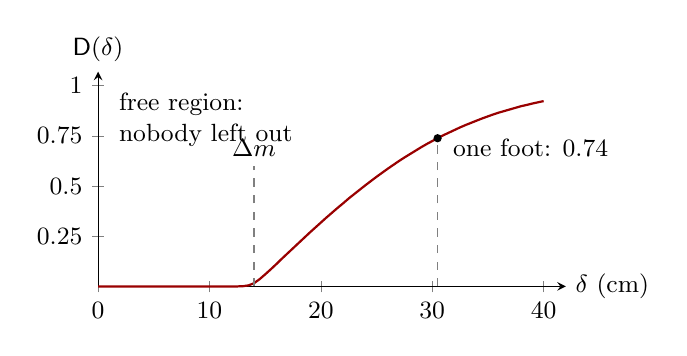
\begin{tikzpicture}[font=\small]
    \begin{axis}[
        scale only axis, width=0.49\textwidth,
        height=0.225\textwidth, clip=false,
        axis lines=left, xmin=0, xmax=42, ymin=0, ymax=1.07,
        xtick={0,10,20,30,40}, ytick={0.25,0.5,0.75,1},
        xlabel={$\delta$ (cm)}, ylabel={$\D(\delta)$},
        x label style={at={(axis description cs:1,0)}, anchor=west},
        y label style={at={(axis description cs:0,1)}, anchor=south,
        rotate=-90},
      ]
      % sup_t (G_W(t) - G_M(t+delta))^+ for N(175.3, 7.6^2) vs
      % N(161.3, 7.1^2), maximised over a 0.02 cm grid in t
      \addplot[thick, red!60!black] coordinates {
        (0,0) (12.5,0) (13,0.001) (13.5,0.005) (14,0.016) (14.5,0.036)
        (15,0.060) (15.5,0.085) (16,0.111) (16.5,0.138) (17,0.164) (17.5,0.190)
        (18,0.216) (18.5,0.242) (19,0.268) (19.5,0.293) (20,0.318) (20.5,0.343)
        (21,0.367) (21.5,0.391) (22,0.414) (22.5,0.438) (23,0.460) (23.5,0.482)
        (24,0.504) (24.5,0.525) (25,0.546) (25.5,0.566) (26,0.586) (26.5,0.605)
        (27,0.624) (27.5,0.642) (28,0.659) (28.5,0.676) (29,0.693) (29.5,0.709)
        (30,0.724) (30.5,0.739) (31,0.753) (31.5,0.766) (32,0.779) (32.5,0.792)
        (33,0.804) (33.5,0.815) (34,0.826) (34.5,0.837) (35,0.847) (35.5,0.857)
        (36,0.866) (36.5,0.874) (37,0.882) (37.5,0.890) (38,0.898) (38.5,0.904)
        (39,0.911) (39.5,0.917) (40,0.923)
      };

      \draw[dashed, gray] (14,0) -- (14,0.6) node[above, black] {$\Delta m$};
      \draw[dashed, gray] (30.48,0) -- (30.48,0.738);
      \fill (30.48,0.738) circle (1.5pt);
      \node[anchor=west] at (31,0.69) {one foot: 0.74};
      \node[anchor=west, align=left] at (1,0.83)
      {free region:\\nobody left out};
    \end{axis}
  \end{tikzpicture}
  \caption{Minimal fraction of $\W$ left unmatched as a function of
    the required height gap, US calibration with unequal variances.
  Essentially zero until about 13 cm, then roughly 5\% per centimeter.}
\end{figure}

\begin{theorem}[The Six-Foot Theorem]\label{thm:sixfoot}
  Suppose a fraction $\alpha$ of $\W$ requires $s(x)\ge\tau$, and
  everyone else imposes any constraint whatsoever. Then at least
  $(\alpha - G_\M(\tau))^+$ of $\W$ is unmatched in every feasible
  matching. For $\tau = 182.9$~\textup{cm} (six feet),
  $G_\M(\tau)\approx0.16$.
\end{theorem}

\begin{proof}
  The constrained set $A$ has neighborhood inside $\{s\ge\tau\}$, of
  mass $G_\M(\tau)$. Apply the Hall bound from Theorem~\ref{thm:deficit}.
\end{proof}

\begin{remark}
  Theorem~\ref{thm:sixfoot} holds regardless of personality, effort,
  or app. It is also generous: it assumes every six-footer is
  available and interested.
\end{remark}

\newpage % start Section 4 on a new page
\section{The Blackpill Theorems}\label{sec:blackpill}

\begin{lemma}[Conservation of Status]\label{lem:status}
  If $s\in L^1(\mu)\cap L^1(\nu)$, then for every
  $\pi\in\Pi(\mu,\nu)$, $\int(s(x)-s(y))\,d\pi = \int t\,d\mu_s -
  \int t\,d\nu_s$. The average status gap across all couples does not
  depend on who marries whom.
\end{lemma}

\begin{proof}
  Integrate against $\pi$ and use its marginals.
\end{proof}

\begin{definition}[Strategy]\label{def:strategy}
  A \emph{strategy} is any map
  $\mathfrak{S}:\Pi(\mu,\nu)\to\Pi(\mu,\nu)$: every intervention that
  changes who matches with whom without changing the population. This
  includes openers, dating apps, ``just be confident,'' and every
  other object the literature calls \emph{cope}.
\end{definition}

\begin{theorem}[Cope Invariance]\label{thm:cope}
  If $\Psi:\Pi(\mu,\nu)\to\R$ depends on $\pi$ only through its
  marginals, then $\Psi\circ\mathfrak{S} = \Psi$ for every strategy
  $\mathfrak{S}$. In particular the mean status gap, the feasibility
  of universal hypergamy, the deficit $\D$, and the equilibrium index
  $\Hy^*$ of \eqref{eq:index} are invariant under every strategy.
\end{theorem}

\begin{proof}
  Strategies preserve marginals, and each listed quantity is a
  functional of $(\mu_s,\nu_s)$ alone.
\end{proof}

\begin{corollary}[It's Over]\label{cor:over}
  If $\mu_s = \nu_s$, no strictly hypergamous matching exists and no
  strategy produces one: by Lemma~\ref{lem:status} applied to the
  bounded status $\arctan s$, the integrand $\arctan s(x)-\arctan s(y)$
  would be positive $\pi$-a.e.\ with zero integral.
\end{corollary}

The only escape is to change the marginals, replacing $s$ by $s+h$
with $h\ge0$ on a subset of agents. We call this \emph{maxxing}.

\begin{theorem}[Conservation of Rank]\label{thm:rank}
  Let $F_\M, F_\W$ be continuous and let the market clear at the
  comonotone coupling. If $U = F_\M(s(x))$ is an agent's own quantile
  and $V = F_\W(s(y))$ their partner's, then $V = U$ a.s.\ and
  $U\sim\Unif(0,1)$. Hence for any perturbation $s\mapsto s+h$ that
  keeps $F_\M$ and $F_\W$ continuous, maxxing included,
  \begin{equation}
    \mathbb{E}[V] = \tfrac12, \qquad \Var(V) = \tfrac1{12}
  \end{equation}
  before and after. Maxxing by a subpopulation raises its partners'
  quantiles by exactly the amount it lowers everyone else's.
\end{theorem}

\begin{proof}
  Under the comonotone coupling $s(y) = F_\W^{-1}(F_\M(s(x)))$, so $V
  = U$. The probability integral transform gives $U\sim\Unif(0,1)$
  for any continuous $F_\M$, perturbed or not.
\end{proof}

\begin{tcolorbox}[colback=white, colframe=black!50, boxrule=0.5pt]
  \textbf{Remark (The Blackpill, Stated Precisely).}
  Theorems~\ref{thm:cope} and~\ref{thm:rank} are the rigorous content
  of ``it's over'': aggregate outcomes are pinned by the marginals,
  strategies act within a fiber of fixed marginals, and status gains
  are transfers of rank, not creation of it. But both are statements
  about the \emph{population}. For an individual at quantile $u$ the
  comonotone map is strictly increasing, so raising your own status
  raises your partner's quantile one-for-one, and for $\theta > 0$
  (Section~\ref{sec:taste}) outcomes are random rather than determined.

  \begin{center}
    \bfseries It is over for the population. It is not over for you.
  \end{center}
\end{tcolorbox}

\section{Everyone Wants Up, Almost Everyone Goes Down}

Take finite sides $|\M| = |\W| = n$ with distinct statuses and
\emph{status-ranked} preferences: every agent strictly prefers a
higher-status partner, and any partner to none. A matching is
\emph{stable} if no pair would both rather be with each other than
with their assigned partners.

\begin{theorem}[Uniqueness of the Assortative Equilibrium]\label{thm:gs}
  Under status-ranked preferences the unique stable matching pairs
  the $k$-th highest of $\M$ with the $k$-th highest of $\W$ for
  every $k$, and Gale--Shapley deferred acceptance~\cite{gale}
  returns it whichever side proposes.
\end{theorem}

\begin{proof}
  Induct on $n$. If the two top agents are not matched to each other,
  they form a blocking pair. Remove them; the reduced market has the
  same structure.
\end{proof}

\begin{corollary}[Everyone Wants Up, Almost Everyone Goes Down]
  In Example~\ref{ex:beta} the assortative matching is the quantile
  map $T = F_\M^{-1}\circ F_\W$, $T(b) = b^2 < b$ on $(0,1)$, and no
  pair blocks it: a man at quantile $u$ prefers a woman at quantile $v$
  only if $v > u$, and she prefers him only if $u > v$. Hence $\Hy = 0$
  and $\Hy^{\downarrow} = 1$: every member of $\W$ prefers to marry up,
  the market is stable, and almost every member of $\W$ marries down,
  by an average of $\int_0^1 (b-b^2)\,2b\,db = \frac16$.
\end{corollary}

\section{Transferable Utility and Optimal Transport}

Following Becker~\cite{becker} and Shapley--Shubik~\cite{shapley}, a
couple with statuses $a$ and $b$ generates surplus $f(a,b)$, which
partners may split. The equilibrium solves the Monge--Kantorovich
problem
\begin{equation}\label{eq:mk}
  \sup_{\pi\in\Pi(\mu,\nu)} \int f(s(x),s(y))\,d\pi =
  \inf_{u(x)+v(y)\,\ge\,f(s(x),s(y))}
  \left\{\int u\,d\mu + \int v\,d\nu\right\},
\end{equation}
where equality is Kantorovich duality and $(u,v)$ are the equilibrium
utilities~\cite{villani}.

\begin{theorem}[Becker via Cyclical Monotonicity]\label{thm:becker}
  If $f$ is strictly supermodular ($\partial_{ab}f > 0$), every
  optimal plan has status projection equal to the comonotone coupling
  $\gamma^* = (F_\M^{-1},F_\W^{-1})_\#\Unif(0,1)$.
\end{theorem}

\begin{proof}
  Optimal plans are cyclically monotone. If $a_1 < a_2$ and $b_1 >
  b_2$ were both in the support, then
  \begin{equation}
    f(a_2,b_1) + f(a_1,b_2) - f(a_1,b_1) - f(a_2,b_2) =
    \int_{a_1}^{a_2}\!\int_{b_2}^{b_1} \partial_{ab}f\,d\beta\,d\alpha > 0,
  \end{equation}
  so swapping partners strictly improves total surplus, a contradiction.
\end{proof}

So bargaining or not, the realized hypergamy index is the same:
\begin{equation}\label{eq:index}
  \Hy^* := \Hy(\gamma^*) = \Leb\{u\in(0,1) : F_\M^{-1}(u) > F_\W^{-1}(u)\}.
\end{equation}

\section{Taste Heterogeneity: The Entropic Relaxation}\label{sec:taste}

Real agents are not perfectly status-ranked. Following Choo and
Siow~\cite{choo} and Galichon and Salani\'e~\cite{galichon}, add
i.i.d.\ Gumbel taste shocks of scale $\theta > 0$. With finitely many
types, write $f_{ij}$ for the surplus of a type-$i$ man with a type-$j$
woman. Equilibrium couples $\pi_{ij}$ and singles $\pi_{i0},\pi_{0j}$
satisfy
\begin{equation}
  \pi_{ij} = \sqrt{\pi_{i0}\pi_{0j}}\,e^{f_{ij}/(2\theta)},
\end{equation}
the first-order conditions of the entropy-regularized problem
\begin{equation}
  \max_{\pi\ge0} \Big\{\sum_{i,j}f_{ij}\pi_{ij} -
  \theta\Ent(\pi)\Big\}, \qquad \Ent(\pi) =
  2\sum_{i,j}\pi_{ij}\log\pi_{ij} + \sum_i\pi_{i0}\log\pi_{i0} +
  \sum_j\pi_{0j}\log\pi_{0j},
\end{equation}
subject to the population constraints. Writing $a_i =
\sqrt{\pi_{i0}}$, $b_j = \sqrt{\pi_{0j}}$, $K_{ij} =
e^{f_{ij}/(2\theta)}$, these become $a_i^2 + a_i(Kb)_i = \mu_i$ and
$b_j^2 + b_j(K^\top a)_j = \nu_j$, solved alternately in closed form
by a generalized iterative proportional fitting procedure.

\begin{theorem}[Vanishing and Exploding Taste]\label{thm:taste}
  Let the market be balanced and $f$ strictly supermodular. If every
  $f_{ij} > 0$, then as $\theta\downarrow0$ the equilibrium converges
  to an optimal plan of \eqref{eq:mk} and $\Hy\to\Hy^*$. In the variant
  without singles this holds for any sign of $f_{ij}$, and as
  $\theta\to\infty$ the equilibrium converges to $\mu\otimes\nu$ and
  $\Hy\to\mathbb{P}(S_\M > S_\W)$ for independent $S_\M\sim\mu_s$,
  $S_\W\sim\nu_s$.
\end{theorem}

\begin{proof}[Sketch]
  $\Gamma$-convergence of the regularized objectives on a compact
  feasible set. If every $f_{ij} > 0$, a man and a woman left single
  can be matched for a gain, so limit plans have no singles, and
  Theorem~\ref{thm:becker} fixes their status projection, on which
  $\Hy$ depends; for $\theta\to\infty$ the entropy term dominates and
  its unique minimizer over $\Pi(\mu,\nu)$ is the product measure.
\end{proof}

In Example~\ref{ex:beta} the endpoints are $\Hy^* = 0$ and
$\mathbb{P}(S_\M > S_\W) = \frac13$. For height, they are $\Hy^* = 1$
and $\Phi(\Delta m/\sqrt{\sigma_\M^2+\sigma_\W^2})\approx0.91$.
Caring \emph{less} about status produces \emph{more} marrying up in
the first case. Preferences and outcomes are different objects.

\section{Main Result}

\begin{theorem}[Hypergamy Is Solved]\label{thm:main}
  For any marriage market:
  \renewcommand{\labelenumi}{(\alph{enumi})}
  \begin{enumerate}
    \item universal hypergamy is feasible iff
      $\mu_s\succeq_{\mathrm{FSD}}\nu_s$;
    \item otherwise the minimal unmatched mass is $\D = \sup_t(G_\W - G_\M)^+$;
    \item no strategy changes (a) or (b), and for continuous
      $F_\M,F_\W$ maxxing is zero-sum in rank;
    \item the equilibrium is the comonotone coupling, with index
      ${\Hy^* = \Leb\{F_\M^{-1} > F_\W^{-1}\}}$, under strictly
      supermodular transferable utility and under status-ranked
      preferences in the finite markets of Theorem~\ref{thm:gs};
    \item when taste shocks of scale $\theta$ are added to the
      transferable utility of (d), with finitely many types and no
      singles, the realized index tends to $\Hy^*$ as
      $\theta\downarrow0$ and to $\mathbb{P}(S_\M > S_\W)$ as
      $\theta\to\infty$.
  \end{enumerate}
  Every quantity in (a)--(d) is a functional of $(\mu_s,\nu_s)$ alone,
  and (e) adds only $\theta$ and the surplus $f$. No other behavioral
  input is required.
\end{theorem}

\begin{proof}
  Theorems \ref{thm:feas}, \ref{thm:deficit}, \ref{thm:cope},
  \ref{thm:rank}, \ref{thm:gs}, \ref{thm:becker}, and \ref{thm:taste}.
\end{proof}

\begin{remark}[Interpretation]
  When one side's status distribution overtakes the other's, measured
  hypergamy falls even if no one's preferences change. This matches
  the reversal of the gender gap in education documented by Esteve et
  al.~\cite{esteve}, who report a global shift from educational
  hypergamy toward hypogamy.
\end{remark}

\section{Beyond Height: Multidimensional Status}\label{sec:multi}

Height is one coordinate of a longer list. Let each man carry a trait
vector $x = (x_1,\dots,x_k)$ (height, face, confidence, charisma,
kindness, income, and so on), each coordinate a within-sex $z$-score, so
that $\mu$ is now a distribution on $\R^k$. A requirement can combine
traits in two ways: as a checklist, where every trait must clear its own
bar, or as a trade-off, where strength in one trait offsets weakness in
another.

\begin{theorem}[The Checklist Theorem]\label{thm:checklist}
  Suppose a fraction $\alpha$ of $\W$ requires every trait to clear a
  bar, $x\in A = \{x_1\ge\tau_1,\dots,x_k\ge\tau_k\}$. Then at least
  $(\alpha-\mu(A))^+$ of $\W$ is unmatched in every feasible matching,
  and for independent traits $\mu(A) = \prod_i\mu(x_i\ge\tau_i)$.
\end{theorem}

\begin{proof}
  The constrained women's neighborhood lies inside $A$, of mass
  $\mu(A)$. Apply the Hall bound from Theorem~\ref{thm:deficit}, exactly
  as in Theorem~\ref{thm:sixfoot}.
\end{proof}

\begin{example}
  In the calibration of Section~\ref{sec:sixfoot}, six feet is
  $x_1\ge1$, so $\mu(x_1\ge1)\approx0.16$. Adding a top-20\% face and
  top-30\% confidence leaves $\mu(A)\approx0.16\times0.2\times0.3
  \approx0.01$ for independent traits. With a common pairwise
  correlation $\rho$ between traits (a one-factor Gaussian model),
  $\mu(A)$ rises to $0.032$ at $\rho=0.3$ and $0.054$ at $\rho=0.5$.
  For independent traits, bars multiply: every requirement added
  shrinks the eligible pool by its own pass rate. Correlation softens
  this without removing it: at $\rho=0.5$ the face bar keeps 46\% of
  the six-footers, and the confidence bar 73\% of those left.
\end{example}

\begin{proposition}[Compensation]\label{prop:comp}
  If instead $\W$ ranks men by an index $s(x) = \beta\cdot x$, then $s$
  is a scalar status functional, and Theorem~\ref{thm:main} applies to
  it once $s$ is also defined on $\W$ on the same scale. For independent
  standard Gaussian traits, the fraction of the top $\Phi(-c)$ of men by
  index who fall below $c$ on trait $i$ is
  \begin{equation}
    1 - \frac{\Phi_2(-c,-c;r_i)}{\Phi(-c)}, \qquad r_i =
    \frac{\beta_i}{\|\beta\|},
  \end{equation}
  where $\Phi_2(\cdot,\cdot;r)$ is the standard bivariate normal CDF with
  correlation $r$.
\end{proposition}

\begin{proof}
  $(x_i, s/\|\beta\|)$ is standard bivariate normal with correlation
  $r_i$, and the top $\Phi(-c)$ of men by index is the event
  $s/\|\beta\|\ge c$.
\end{proof}

\begin{remark}
  With equal weights on height, face and confidence ($r_i=1/\sqrt3$)
  and $c=1$, take the top 16\% of men by index, as many men as are six
  feet tall: 56\% of them are under six feet. Under a checklist six
  feet is a gate; under a trade-off it is one input among several. The
  Six-Foot Theorem is a statement about the checklist.
\end{remark}

Nothing requires the two sides to be scored on the same traits. Let $\W$
rank men by an index $s_\M$ and $\M$ rank women by a different index
$s_\W$. Scores on different traits share no unit, so compare positions
instead: write $U = F_\M(s_\M(x))$ and $V = F_\W(s_\W(y))$ for each
person's quantile within their own side.

\begin{theorem}[Quantile Hypergamy]\label{thm:quantile}
  In a balanced market with continuous score distributions, if every
  member of $\W$ requires $U\ge V+\delta$, where $0\le\delta\le1$, the
  minimal unmatched mass of $\W$ is exactly $\delta$, whatever traits
  define $s_\M$ and $s_\W$.
\end{theorem}

\begin{proof}
  By the probability integral transform $U$ and $V$ are both
  $\Unif(0,1)$. Shifting by $\delta$ as in Section~\ref{sec:sixfoot},
  Theorem~\ref{thm:deficit} gives $\D(\delta) = \sup_{t\in[0,1]}
  \bigl((1-t) - (1-t-\delta)^+\bigr)^+ = \delta$, attained at every
  $t\in[0,1-\delta]$.
\end{proof}

\begin{remark}
  At $\delta=0$ the two quantile distributions coincide, so by
  Corollary~\ref{cor:over} no strictly hypergamous matching exists. Once
  status means rank, a market in which everyone marries strictly up is
  not rare but impossible: by Lemma~\ref{lem:status}, every rank gained
  is a rank lost elsewhere.
\end{remark}

\section{What Else Matters}\label{sec:matters}

Height is one coordinate of the trait vector of Section~\ref{sec:multi},
which left the weights $\beta$ unspecified. Here is what the evidence
says about the others. In 37 samples from 33 countries, both sexes
ranked kindness and intelligence above physical attractiveness and
earning capacity; men rated good looks as significantly more important
than women did in 34 samples, and women rated good financial prospects
as significantly more important than men did in 36~\cite{buss}. When
designing a long-term partner on a budget, men treat physical
attractiveness as a necessity, women status and resources, and both
kindness and intelligence~\cite{li2002}. For short-term partners, women,
like men, put physical attractiveness first~\cite{li2006}. A review of
the evidence on sex drive finds it stronger in men than in women, with no
contrary findings~\cite{baumeister}.

Stated preferences predict little of what happens next. In speed dating,
the sex differences in the stated importance of looks and earnings do
not appear in whom people actually like, and stated ideals do not
predict it~\cite{eastwick}. Across 43 longitudinal studies of couples,
features of the relationship itself, led by how committed the partner
seems, appreciation, sexual satisfaction, how satisfied the partner seems
and conflict, predict up to 45\% of the variance in relationship quality
at the start of a study and 18\% at the end, against 21\% and 12\% for
individual differences such as mood and attachment style, and neither
individual differences nor the partner's own reports add anything to
what a person reports about the relationship~\cite{joel}. The
relationship itself is the best predictor of how it goes.

Money counts for whoever weights it. Among 6,485 users of an online
dating service in Boston and San Diego, an income of \$150k to \$200k
rather than \$35k to \$50k raised the chance that a woman contacted a man
by 8.9 percentage points, and that a man contacted a woman by 3.9,
though few users, and especially few women, reported incomes that
high~\cite{hitsch}. The same users show what height preferences look like
in practice. Women were much less likely to contact men shorter than
themselves, and a man more than five inches taller, rather than within
two inches of her height, raised a woman's chance of contacting him by
7.1 points, about as much as looks in the 81st to 90th percentile rather
than the bottom decile (7.9). There was no evidence that women cared
about absolute height, and men's preference for women at least 5 foot 3
was small. Height matters, then, as a relative comparison, and the
market can meet it: even as a requirement, five inches is below the mean
difference of about 14 cm and leaves about one woman in eight thousand
unmatched in the calibration of Section~\ref{sec:sixfoot}. It is the
absolute bar of Theorem~\ref{thm:sixfoot} that excludes, and these women
show no sign of one.

Short-term play adds game, which is a strategy in the sense of
Definition~\ref{def:strategy} when it changes who meets whom, and
maxxing when it raises the index itself, since confidence and charisma
are on the list. Either way Theorems~\ref{thm:cope} and~\ref{thm:rank}
bound what it does for the population, and the boxed remark in
Section~\ref{sec:blackpill} says what it does for an individual. For
men, the author emphasizes the teachings of Jake Abdo~\cite{abdo} as
optimal play for short-term dating; optimality is not proved here.

Uncertainty is part of the game. Women told that a man's interest in them
was uncertain were more attracted to him than women told that he liked
them a lot, and thought about him more~\cite{whitchurch}. If someone is
already committed to pursuing you, playing hard to get raises how much
they want you but lowers how much they like you; otherwise it lowers
both~\cite{dai}. A partner's attachment security also predicts
attraction~\cite{klohnen}, which suggests that unavailability at best
trades liking for wanting. Mystery has a shelf life. Learning more about
a person can lower liking~\cite{norton}, though more time in live
conversation raises liking between strangers~\cite{reis}, and among
newlyweds it was disillusionment, a fading of love and affection over the
first two years, that marked the couples headed for divorce~\cite{huston}.
Mystery works like the idealization $\iota$ of Section~\ref{sec:abuse},
applied to a current partner, and information removes it. The
uncertainty finding comes from women only~\cite{whitchurch}; whether it
holds for men is untested there.

In the notation of Section~\ref{sec:multi}, each side ranks the other by
its own index, which Theorem~\ref{thm:quantile} allows, with stated
weights that change with the horizon: kindness and intelligence in the
long run, looks in the short run, and money for whoever is looking for
it. The relationship itself is no one's trait. Its nearest counterpart
in Section~\ref{sec:taste} is the taste shock, the part of the surplus
that status does not explain, although Choo and Siow attach each shock
to a person and a type of partner rather than to a couple. In the
variant without singles, Theorem~\ref{thm:taste} says the equilibrium
tends to random matching as the shocks grow relative to the status
surplus.

\section{Partner History}\label{sec:history}

A common claim holds that fewer previous partners make for better
relationships, either because the capacity to pair-bond gets used up or
because a partner with no history has no one to compare you to. The data
support an association, but not one confined to women. Among 2,654
married individuals, Busby, Willoughby and Carroll~\cite{busby} find
that more lifetime partners go with lower sexual quality, poorer
communication and lower stability, with no significant difference
between men and women. Using longitudinal data on both sexes, Smith and
Wolfinger~\cite{smith} find divorce risk highest with six or more
premarital partners and next highest with one or two, while three to
five do not differ significantly from none besides the eventual spouse;
the link survives controls for religion, values, family relationships,
personality and mental health, shows no gender difference, and
selection is not ruled out.

Wolfinger~\cite{wolfinger} reports the lowest divorce rates for women
with zero or one premarital partners, an irregular pattern above that,
and religiosity as part of the explanation for the low end; that
analysis covers only women because the survey lacks full data on men's
premarital sex. The neurobiology of pair bonding comes from studies of
monogamous rodents~\cite{young}, and its human version, in which bonding
capacity is used up by previous partners, has not been established. We
therefore treat partner history as a hypothesis, and treat it
symmetrically.

\begin{definition}[Comparison]\label{def:comparison}
  A person whose previous partners had qualities $Q_1,\dots,Q_n$, drawn
  i.i.d.\ from a distribution $F$ with finite mean, values a new partner
  of quality $q$ at $q - \lambda(M_n-q)^+$, where $M_n = \max_{i\le n}
  Q_i$, $M_0 = -\infty$, and $\lambda\ge0$ measures how much comparison
  matters. Only an ex who was better than the new partner costs
  anything.
\end{definition}

\begin{proposition}[Diminishing Comparisons]\label{prop:comparison}
  The expected regret $R_n(q) = \mathbb{E}[(M_n-q)^+]$ is increasing and
  concave in $n$, with $R_0 = 0$ and
  \begin{equation}
    R_{n+1}(q) - R_n(q) = \int_q^\infty F(t)^n\bigl(1-F(t)\bigr)\,dt.
  \end{equation}
  For standard Gaussian quality and an average new partner ($q=0$),
  $R_n = 0$, $0.40$, $0.68$, $0.89$, $1.17$, $1.54$, $1.87$ at $n = 0$,
  $1$, $2$, $3$, $5$, $10$, $20$.
\end{proposition}

\begin{proof}
  $R_n(q) = \int_q^\infty\mathbb{P}(M_n>t)\,dt = \int_q^\infty
  \bigl(1-F(t)^n\bigr)\,dt$, which is finite because $F$ has a finite
  mean. Subtract consecutive terms; the integrand $F^n(1-F)$ is
  nonnegative and decreasing in $n$ because $0\le F\le1$.
\end{proof}

\begin{remark}
  The first partner sets the bar and each later one raises it by less,
  so the largest single step is from none to one, though later partners
  still add most of the total: the first supplies 45\% of $R_3$ and
  21\% of $R_{20}$. This fits Wolfinger's jump from one premarital
  partner, usually the husband, to two~\cite{wolfinger}, but not his
  higher divorce rate at two than at three to nine, nor Smith and
  Wolfinger~\cite{smith}, whose results suggest a link that grows
  stronger, not weaker, as partners accumulate. The model cannot tell
  comparison apart from selection, and nothing in it refers to sex: a
  man with many previous partners compares too. If partner history
  enters a status index, Theorem~\ref{thm:rank} applies unchanged: it
  re-sorts who ranks where, and every rank one person gains, someone
  else loses.
\end{remark}

\section{Abusive Partners}\label{sec:abuse}

Definition~\ref{def:comparison} charges nothing for a bad ex, since only
an ex who was better than the new partner costs anything. An abusive ex
can still cost something by being remembered as better than they were.
``Narcissistic abuse'' is not a clinical diagnosis, and the studies
below rate a partner's traits through the person they abused. Among 436
people close to someone high in narcissistic traits, mostly current or
former partners, Day, Townsend and Grenyer~\cite{day} find abuse
alongside mutual idealization and devaluation. Among 75 women who had
just left abusive partners, Dutton and Painter~\cite{dutton} find
attachment to the former partner predicted by how extreme and
intermittent the maltreatment was and by the imbalance of power, both at
separation and six months later.
Among 1,294 people recruited through online communities about narcissism
and abuse, 94\% of them women, Arabi~\cite{arabi} finds that a former
partner's narcissism predicts symptoms of post-traumatic stress, which
include intrusive memories, beyond the frequency of the abuse and any
earlier abuse.

\begin{definition}[Idealization]
  A previous partner is \emph{idealized by} $\iota\ge0$ if they are
  remembered at quality $Q_i+\iota$. With one idealized partner the
  comparison point is $M_n^\iota = \max(Q_1+\iota,Q_2,\dots,Q_n)$, and
  since the $Q_i$ are i.i.d.\ it does not matter which partner it was.
  Write $R_n^\iota(q) = \mathbb{E}[(M_n^\iota-q)^+]$.
\end{definition}

\begin{proposition}[Idealization Compounds]\label{prop:ideal}
  $R_n^\iota(q)$ is nondecreasing and convex in $\iota$, with $R_n^0 =
  R_n$ and $R_1^\iota(q) = R_1(q-\iota)$. For standard Gaussian quality
  and an average new partner ($q=0$), $R_1^\iota = \iota\,\Phi(\iota) +
  \varphi(\iota)$. At $\iota = 1$ this is $1.08$, which is $2.7$ times
  $R_1$ and exceeds $R_4 = 1.05$, the regret from four ordinary previous
  partners; at $\iota = 1.5$ it is $1.53$, almost $R_{10} = 1.54$.
\end{proposition}

\begin{proof}
  Write $M_n^\iota = \max(Q_1+\iota, M')$ with $M'$ free of $\iota$. It
  is convex and nondecreasing in $\iota$, and composing with the convex
  nondecreasing map $x\mapsto(x-q)^+$ preserves both properties; take
  expectations, which are finite because $F$ has a finite mean. Also
  $(Q_1+\iota-q)^+ = (Q_1-(q-\iota))^+$. For $Z\sim N(0,1)$, since
  $\varphi'(z) = -z\varphi(z)$, $\mathbb{E}[(Z+\iota)^+] =
  \int_{-\iota}^\infty (z+\iota)\varphi(z)\,dz = \varphi(\iota) +
  \iota\,\Phi(\iota)$.
\end{proof}

Partners have diminishing returns (Proposition~\ref{prop:comparison})
and idealization has increasing ones, so in this model one idealized ex
can outweigh several ordinary ones, and abuse need not act through $n$
at all. The expected cost of comparison is $\lambda R_n^\iota(q)$, so if
abuse also raises $\lambda$, as the attachment findings suggest, it
multiplies all of the above. No study measures $\iota$. Nothing in the
model refers to sex, although the samples in~\cite{day}, \cite{dutton}
and~\cite{arabi} are mostly or entirely women.

\begin{remark}[First Partners]
  Since it does not matter which partner was idealized, what is special
  about a first partner lies outside the model. While that relationship
  lasts, $M_0 = -\infty$: there is no one to compare them with. Abuse may
  also lower the floor. Thibaut and Kelley's comparison
  level~\cite{thibaut}, the standard a relationship is judged against, is
  learned from experience, and Definition~\ref{def:comparison} has a
  ceiling, $M_n$, but no floor. Among 5,681 adolescents aged 12 to 18,
  dating violence was followed five years later by 1.9 to 3.6 times the
  adjusted odds of being a victim of partner violence, in both sexes, and
  psychological violence alone roughly doubled them~\cite{exner}. This
  fits a lowered floor, but selection is not ruled out.
\end{remark}

\begin{remark}[Recovery]
  None of this need be permanent. In~\cite{dutton}, attachment to the
  former partner fell by about 27\% over the six months, so $\lambda$ is
  better read as decreasing in the time since the relationship ended. An
  inability to experience loving feelings is a listed symptom of
  post-traumatic stress disorder~\cite{dsm}, which needs no appeal to the
  used-up bonding capacity of Section~\ref{sec:history}. After breakups in
  general, not only abusive ones, sex to cope with distress or to get back
  at the ex is most frequent soon after the breakup and then
  declines~\cite{barber}.
\end{remark}

\begin{remark}[Flipping]
  A survivor is sometimes said to flip hypergamy and seek a partner of
  lower status. That is hypergamy for the status functional $-s$, so
  every theorem above applies with $-s$ in place of $s$, and by
  Theorem~\ref{thm:deficit} the deficit becomes $\sup_t(\nu(s\le
  t)-\mu(s\le t))^+$. By Proposition~\ref{prop:crossing}, ``he must be
  taller than me'' is feasible for everyone, but in the calibration of
  Section~\ref{sec:sixfoot}, if all of $\W$ requires ``he must not be
  taller than me,'' about two thirds of $\W$ must stay unmatched. Every
  union in which one partner marries down is one in
  which the other marries up. Whether survivors flip at all is not
  established. The nearest evidence concerns dominance rather than
  status, and depends on where the danger comes from: Colombian women who
  perceive more risk of domestic violence prefer less masculine Colombian
  faces~\cite{borras}, while American women more afraid of crime prefer
  more aggressive and formidable mates~\cite{snyder}.
\end{remark}

\section{Conclusion}

Hypergamy reduces to optimal transport on the real line. Its
feasibility is stochastic dominance, its failure is the Hypergamy
Deficit, its equilibrium is the quantile coupling, and its realized
rate is the measure of the set where one quantile function exceeds
another. Section~\ref{sec:multi} extends the deficit to several traits,
where checklist requirements multiply when traits are independent and
trade-offs reduce to a scalar index, and Section~\ref{sec:matters}
reviews the evidence on the weights: stated preferences put kindness and
intelligence first for the long run and looks first for the short run,
money counts for whoever wants it, the relationship itself best predicts
how it goes, and height enters as a relative comparison the market can
satisfy. Section~\ref{sec:history} treats partner history as a
comparison effect that applies to both sexes, and
Section~\ref{sec:abuse} models an abusive ex as an idealized one, whose
cost compounds where that of additional partners diminishes
(Proposition~\ref{prop:ideal}). Open
problems include general multidimensional status (Brenier
maps and upper sets in a partial order), search frictions, and the case
in which the status functional is itself endogenous.

\paragraph*{Acknowledgments.} The author thanks Zhang et al.\ for
contributions that were substantial but unspecified. \emph{Conflict
of interest:} the author is a participant in the market under study.

\begin{thebibliography}{99}
  \bibitem{abdo} J.~Abdo, @thejakeabdo, Instagram,
  \url{https://www.instagram.com/thejakeabdo/}, accessed October 28,
  2026.
  \bibitem{dsm} American Psychiatric Association, \emph{Diagnostic and
  Statistical Manual of Mental Disorders}, 5th ed., American Psychiatric
  Publishing, 2013.
  \bibitem{arabi} S.~Arabi, Narcissistic and psychopathic traits in
  romantic partners predict post-traumatic stress disorder symptomology:
  Evidence for unique impact in a large sample, \emph{Personality and
  Individual Differences} 201, 2023.
  \bibitem{barber} L.~L. Barber and M.~L. Cooper, Rebound sex: Sexual
  motives and behaviors following a relationship breakup, \emph{Archives
  of Sexual Behavior} 43(2), 2014.
  \bibitem{baumeister} R.~F. Baumeister, K.~R. Catanese, and K.~D. Vohs,
  Is there a gender difference in strength of sex drive? Theoretical
  views, conceptual distinctions, and a review of relevant evidence,
  \emph{Personality and Social Psychology Review} 5(3), 2001.
  \bibitem{becker} G.~S. Becker, A theory of marriage: Part I,
  \emph{Journal of Political Economy} 81(4), 1973.
  \bibitem{borras} M.~L. Borras-Guevara, C.~Batres, and D.~I. Perrett,
  Domestic violence shapes Colombian women's partner choices,
  \emph{Behavioral Ecology and Sociobiology} 71(12), 2017.
  \bibitem{busby} D.~M. Busby, B.~J. Willoughby, and J.~S. Carroll,
  Sowing wild oats: Valuable experience or a field full of weeds?
  \emph{Personal Relationships} 20(4), 2013.
  \bibitem{buss} D.~M. Buss, Sex differences in human mate preferences:
  Evolutionary hypotheses tested in 37 cultures, \emph{Behavioral and
  Brain Sciences} 12(1), 1989.
  \bibitem{choo} E.~Choo and A.~Siow, Who marries whom and why,
  \emph{Journal of Political Economy} 114(1), 2006.
  \bibitem{dai} X.~Dai, P.~Dong, and J.~S. Jia, When does playing hard to
  get increase romantic attraction? \emph{Journal of Experimental
  Psychology: General} 143(2), 2014.
  \bibitem{day} N.~J.~S. Day, M.~L. Townsend, and B.~F.~S. Grenyer,
  Pathological narcissism: An analysis of interpersonal dysfunction
  within intimate relationships, \emph{Personality and Mental Health}
  16(3), 2022.
  \bibitem{dutton} D.~G. Dutton and S.~Painter, Emotional attachments in
  abusive relationships: A test of traumatic bonding theory,
  \emph{Violence and Victims} 8(2), 1993.
  \bibitem{eastwick} P.~W. Eastwick and E.~J. Finkel, Sex differences in
  mate preferences revisited: Do people know what they initially desire
  in a romantic partner? \emph{Journal of Personality and Social
  Psychology} 94(2), 2008.
  \bibitem{esteve} A.~Esteve, C.~R. Schwartz, J.~Van Bavel,
  I.~Permanyer, M.~Klesment, and J.~Garc\'{\i}a-Rom\'an, The end of
  hypergamy: Global trends and implications, \emph{Population and
  Development Review} 42(4), 2016.
  \bibitem{exner} D.~Exner-Cortens, J.~Eckenrode, and E.~Rothman,
  Longitudinal associations between teen dating violence victimization
  and adverse health outcomes, \emph{Pediatrics} 131(1), 2013.
  \bibitem{fryar} C.~D. Fryar, M.~D. Carroll, Q.~Gu, J.~Afful, and
  C.~L. Ogden, Anthropometric reference data for children and adults:
  United States, 2015--2018, \emph{Vital and Health Statistics}
  Series 3, No.~46, National Center for Health Statistics, 2021.
  \bibitem{gale} D.~Gale and L.~S. Shapley, College admissions and
  the stability of marriage, \emph{American Mathematical Monthly} 69(1), 1962.
  \bibitem{galichon} A.~Galichon and B.~Salani\'e, Cupid's invisible
  hand: Social surplus and identification in matching models,
  \emph{Review of Economic Studies} 89(5), 2022.
  \bibitem{hitsch} G.~J. Hitsch, A.~Horta\c{c}su, and D.~Ariely, What
  makes you click? Mate preferences in online dating, \emph{Quantitative
  Marketing and Economics} 8(4), 2010.
  \bibitem{huston} T.~L. Huston, J.~P. Caughlin, R.~M. Houts, S.~E. Smith,
  and L.~J. George, The connubial crucible: Newlywed years as predictors
  of marital delight, distress, and divorce, \emph{Journal of Personality
  and Social Psychology} 80(2), 2001.
  \bibitem{joel} S.~Joel, P.~W. Eastwick, C.~J. Allison, et al., Machine
  learning uncovers the most robust self-report predictors of
  relationship quality across 43 longitudinal couples studies,
  \emph{Proceedings of the National Academy of Sciences} 117(32), 2020.
  \bibitem{klohnen} E.~C. Klohnen and S.~Luo, Interpersonal attraction and
  personality: What is attractive---self similarity, ideal similarity,
  complementarity or attachment security? \emph{Journal of Personality and
  Social Psychology} 85(4), 2003.
  \bibitem{li2002} N.~P. Li, J.~M. Bailey, D.~T. Kenrick, and
  J.~A.~W. Linsenmeier, The necessities and luxuries of mate preferences:
  Testing the tradeoffs, \emph{Journal of Personality and Social
  Psychology} 82(6), 2002.
  \bibitem{li2006} N.~P. Li and D.~T. Kenrick, Sex similarities and
  differences in preferences for short-term mates: What, whether, and
  why, \emph{Journal of Personality and Social Psychology} 90(3), 2006.
  \bibitem{norton} M.~I. Norton, J.~H. Frost, and D.~Ariely, Less is more:
  The lure of ambiguity, or why familiarity breeds contempt,
  \emph{Journal of Personality and Social Psychology} 92(1), 2007.
  \bibitem{reis} H.~T. Reis, M.~R. Maniaci, P.~A. Caprariello,
  P.~W. Eastwick, and E.~J. Finkel, Familiarity does indeed promote
  attraction in live interaction, \emph{Journal of Personality and Social
  Psychology} 101(3), 2011.
  \bibitem{shapley} L.~S. Shapley and M.~Shubik, The assignment game
  I: The core, \emph{International Journal of Game Theory} 1(1), 1971.
  \bibitem{smith} J.~Smith and N.~H. Wolfinger, Re-examining the link
  between premarital sex and divorce, \emph{Journal of Family Issues}
  45(3), 2024.
  \bibitem{snyder} J.~K. Snyder, D.~M.~T. Fessler, L.~Tiokhin,
  D.~A. Frederick, S.~W. Lee, and C.~D. Navarrete, Trade-offs in a
  dangerous world: Women's fear of crime predicts preferences for
  aggressive and formidable mates, \emph{Evolution and Human Behavior}
  32(2), 2011.
  \bibitem{strassen} V.~Strassen, The existence of probability
  measures with given marginals, \emph{Annals of Mathematical
  Statistics} 36(2), 1965.
  \bibitem{thibaut} J.~W. Thibaut and H.~H. Kelley, \emph{The Social
  Psychology of Groups}, Wiley, 1959.
  \bibitem{villani} C.~Villani, \emph{Optimal Transport: Old and
  New}, Springer, 2009.
  \bibitem{whitchurch} E.~R. Whitchurch, T.~D. Wilson, and D.~T. Gilbert,
  ``He loves me, he loves me not \ldots'': Uncertainty can increase
  romantic attraction, \emph{Psychological Science} 22(2), 2011.
  \bibitem{wolfinger} N.~H. Wolfinger, Counterintuitive trends in the
  link between premarital sex and marital stability, Institute for
  Family Studies, June 6, 2016.
  \bibitem{young} L.~J. Young and Z.~Wang, The neurobiology of pair
  bonding, \emph{Nature Neuroscience} 7(10), 2004.
\end{thebibliography}

\end{document}
